\section{Besoins fonctionnels}
Lors de nos différents échanges avec le client nous avons pu identifier ses besoins pour ce projet. En effet, la réalisation de ce projet nécessite plusieurs parties:

\subsection{Partie Langue}
Mettre en place une base de données qui utilise le niveau intensif du \textbf{LeFFF} pour former les différents mots du \textbf{lexique}.

\subsubsection{Rechercher un lexique - Importance 5/5}

{Nous offrirons la possibilité de rechercher un \textbf{lexique} de la même manière qu'un dictionnaire, mais aussi en permettant de le chercher en fonction de son \textbf{lemme} et \textbf{lexème} (sa définition ou synonyme). Par exemple l'entrée en recherche "content", nous pourrons retrouver en sortie "content", "heureux", "être à la fête", "être aux anges", "être gai comme un pinson",... Par la suite, nous pourrons afficher toutes les formes possibles pour chacun des résultats retournés comme par exemple singulier, pluriel, ou temps conjugués pour les verbes. Un exemple de test réalisable serait de rechercher un mot et de refaire une recherche avec l'un des résultats obtenus pour comparer les deux recherches.\par}

\begin{figure}[h]
    \centering
    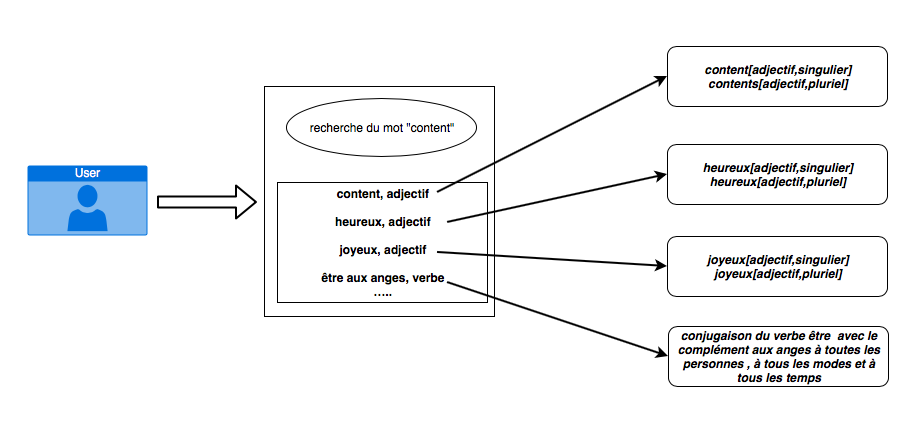
\includegraphics[scale=0.5]{exemple.png}
    \caption{Scénario d'utilisation pour la recherche d'un mot }
\end{figure}
\newpage

\subsubsection{Transducteur - Importance 5/5}


La composition des \textbf{transducteurs} nous permettra de construire un \textbf{lexique} spécifique à la nature de l'entrée, nous pouvons réaliser des \textbf{transducteurs} par exemple qui vont \textbf{conjuguer} des verbes, d'autres qui vont \textbf{transformer} du masculin ou féminin, du singulier ou pluriel, ou \textbf{inversement}. Les algorithmes de construction des transducteurs pourront prendre en compte des \textbf{filtres} afin d'affiner la recherche et la rendre plus rapide.Chaque \textbf{arcs} correspondra à une \textbf{spécification} du mot (symboles signifiant la nature et la morphologie d'un mot).



{Il faudra mettre en place un transducteur qui aura pour fonction de récupérer le radical d'un mot fourni pour se faire nous utiliserons plusieurs automates finis afin de détecter sa catégorie grammaticale, pour ensuite connaître sa forme dans le but de retourner son radical.}

{Inversement, à partir d'un autre transducteur, celui ci devra retourner toutes ses formes.}

\begin{figure}[ht]
    \centering
    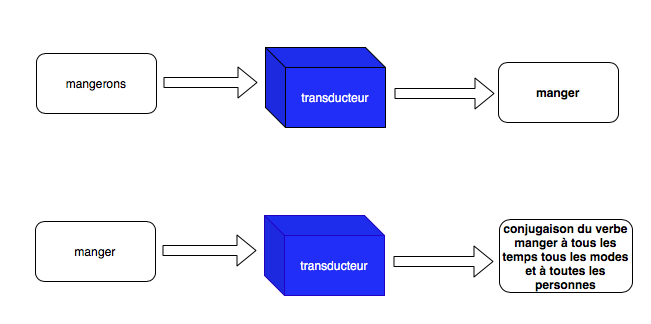
\includegraphics[scale=0.5]{transducteur.png}
    \caption{transducteur }
\end{figure}
\subsubsection{Base de Données - Importance 5/5}


{Nous allons utiliser une \textbf{base de données relationnelle}. A première vue il aurait été plus judicieux d'utiliser une base de données non relationnelle du fait du nombre volumineux de données à traiter. Néanmoins le choix d'utiliser ici une base de données relationnelle nous permettra une plus \textbf{simple} gestion des données en particulier pour la recherche. Afin \textbf{d'optimiser} la \textbf{recherche} nous utiliserons une ou plusieurs de ces 3 solutions : 
\begin{itemize}
\item Des \textbf{fichiers triés}, rapide pour la recherche (recherche dichotomique), mais lents pour l'insertion et la suppression.
\item Des \textbf{fichiers hachés} efficaces pour les sélections avec égalité.
\item Des \textbf{index} (pour chaque lettre de l'alphabet) pour permettre d'améliorer certaines opérations sur un fichier.
\end{itemize}\par}


\subsubsection{Unificateur - Importance 5/5}{
\textbf{L'unificateur} est l'algorithme qui va nous permettre de \textbf{lier} plusieurs \textbf{mots} afin d'en tirer le \textbf{sens}, pour ce faire, il faut faire \textbf{l'union des informations} sur ces mots. S'il y a une \textbf{contradiction} avec ces informations, alors la phrase est \textbf{mal formée} et dans ce cas aucun sens ne sera retourné, sinon on pourra voir quel est le sens de l'expression formée.\par}

\begin{figure}[ht]
    \centering
    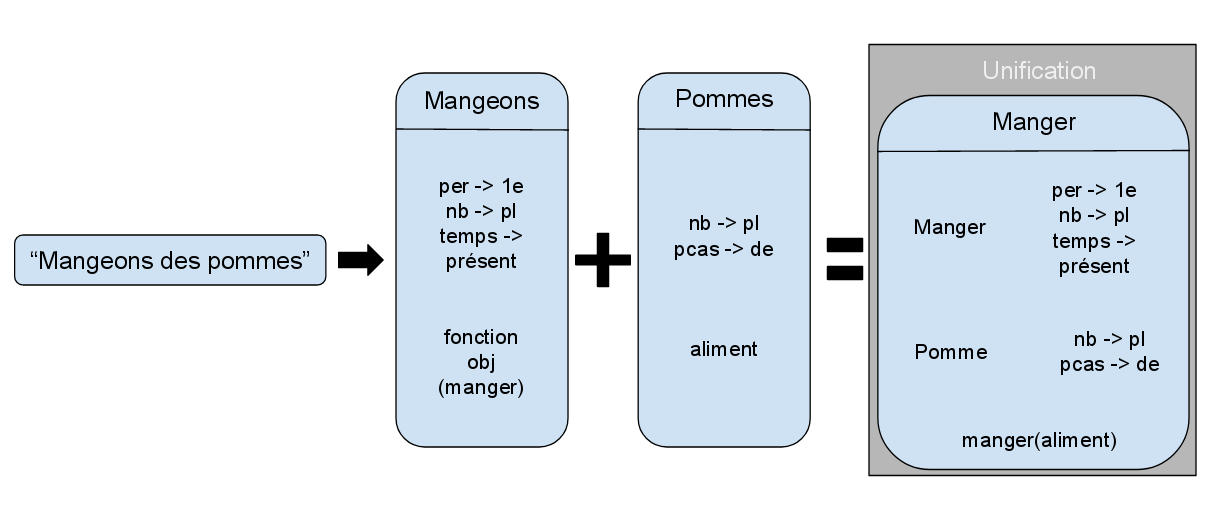
\includegraphics[scale=0.4]{unificateur.png}
    \caption{Unificateur }
\end{figure}

{Les mots utilisés sur \textbf{l'unificateur} utiliserons une \textbf{sous-structure commune} afin de faciliter et de rendre sensée cette opération, puis à l'aide de la \textbf{théorie de substitution des ensembles}, nous pourrons \textbf{optimiser} la construction de nos formules. Celles-ci nous permettrons par la suite d'\textbf{améliorer} la \textbf{rapidité} de l'algorithme de recherche, ainsi que la \textbf{mémoire} utilisée.\par}

\subsection{Partie Web}
Le développement d'une \textbf{application Web} permettant aux utilisateurs de facilement interagir avec le \textbf{lexique}.

\subsubsection{Ajouter un mot au lexique - Importance 4/5}

{Nous offrirons la possibilité d'ajouter un mot au \textbf{lexique} en rentrant les données de la structure du \textbf{FFF} pour celui-ci, c'est à dire que nous devrons entrer des informations sur ce que l'on veut rajouter comme son sens, est-ce un verbe, un nom, un adjectif,..., singulier, pluriel,..., pour pouvoir ensuite être reconnu par l'algorithme de recherche demandé ci-dessus. Un exemple de test réalisable serait de voir si on trouve bien les éléments rajoutés avec la recherche de lexique.\par}

\subsubsection{Supprimer un mot du lexique - Importance 1/5}
{Nous offrirons la possibilité de supprimer un mot ou expression du \textbf{lexique}, affin de les enlever de toute la base de données utilisée, et donc de faire en sorte à ce que l'algorithme de recherche ne le trouve plus. Cette fonction ne sera normalement que très peu utilisée. Un exemple de test réalisable serait de faire une recherche et par la suite de supprimer un des résultats, pour enfin réitérer la recherche sur tous les résultats pour vérifier que l'élément supprimé est bien supprimé.\par}

\subsubsection{Modifier un mot - Importance 4/5}
 
{Nous offrirons la possibilité de modifier un mot du \textbf{lexique} en modifiant un ou plusieurs champs de la structure du \textbf{FFF} de ce mot. Cette fonction permettra entre autre de corriger des erreurs d'ajout dans le lexique comme par exemple faute d'orthographe, mauvaise catégorisation,... Il sera possible de tester cette fonctionnalité en recherchant l'élément modifié directement et de constater ses changements (toutes les possibilités de changement seront donc a tester).\par} L'algorithme d'unification doit prendre en compte la nouvelle modification afin de mettre à jour le lexique d'une manière automatique.
 
\subsubsection{Gérer les rôles - Importance 2/5}
    
    Nous mettrons en place un système à trois \textbf{types d'utilisateurs}:
    \begin{itemize}
    \item \textbf{Utilisateur}:  peut \textbf{consulter} et extraire le lexique.
    \item \textbf{Contributeur}: peut \textbf{s'inscrir, valider,supprimer} son compte, d'autres part il a la possibilité de \textbf{modifier} le lexique et faire ce que fait un utilisateur,
    \item \textbf{Administrateur}: \textbf{gère les droits} des autres utilisateurs (faire passer certains utilisateurs modérateurs et vis versa) et peut faire ce que fait un modérateur.
    \end{itemize}
    {Cette façon de gérer les rôles reste simple mais efficace qui permettra de limiter au maximum les erreurs dans les ajout d'éléments dans le \textbf{lexique}.\par}
    
    \begin{figure}[ht]
        \centering
        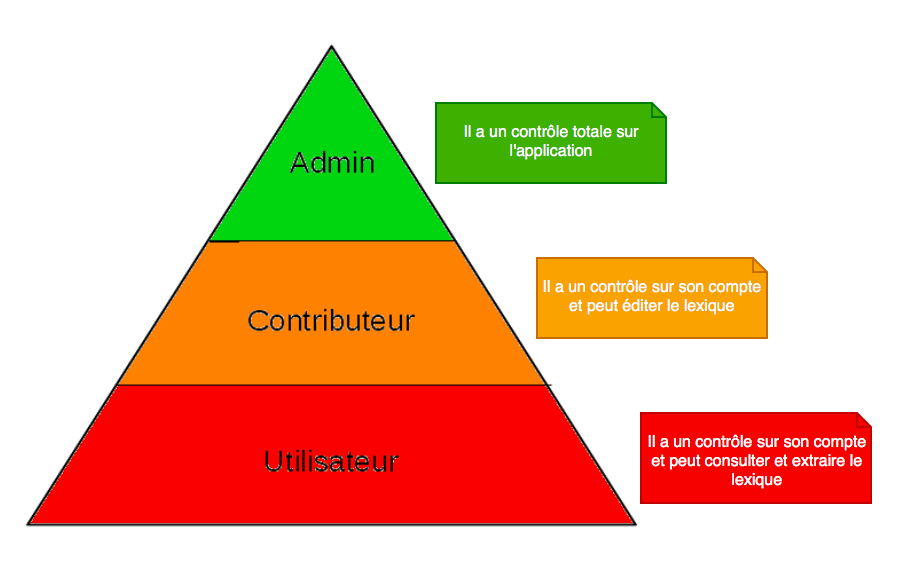
\includegraphics[scale=0.3]{role.png}
        \caption{Gestion des rôles des utilisateurs }
    \end{figure}
    \newpage
    

 
\subsubsection{Exporter le LeFFF - Importance 3/5}
{Nous offrirons la possibilité d'exporter le \textbf{lexique} sélectionné avec un \textbf{filtre} afin que l'utilisateur puisse \textbf{télécharger} un document contenant tous les détails de la recherche, et qui va plus ressembler au format \textbf{Extensif} donné(un format plus lisible), le format choisi est le \textbf{xml} , nous pourrons utiliser plusieurs types de filtres comme une catégorie de mot ou expression (verbe, nom, adjectif,..., singulier, pluriel,...) . Il sera possible de tester cette fonction en exportant sans filtre le \textbf{LeFFF}  et par la suite vérifier que le \textbf{LeFFF} téléchargé est bien entier et au bon format.\par}


\section{Les besoins non fonctionnels}

\subsection{Sécurité}
{Le système doit offrir un \textbf{accès personnalisé} pour nos utilisateurs (chacun à son rôle), de plus doit utiliser des \textbf{protocoles de sécurité} ou des certificats \textsc{Https} }

\subsection{Format de fichier}
Nous offrirons la possibilité de gérer le téléchargement du \textbf{LeFFF} ou d'une partie du \textbf{lexique} sous plusieurs format au choix  \textbf{txt},\textbf{xml}, \textbf{ilex} : pour le radical des mots c'est à dire une version de base pas compilé du leFFF intensif, \textbf{tlex} : format compilé niveau extensif.

\subsection{Performances}

{Nous devrons faire en sorte à ce que la \textbf{base de données} soit \textbf{optimisée} afin qu'une recherche ou exportation par de multiple personnes en même temps ne prenne par un temps trop grand.\par}
Nous sommes dans l'obligation de manipuler la \textbf{gestion de la mémoire} d'une manière très \textbf{efficace} dans le but d'assurer le fonctionnement des besoins fonctionnels dans tous les scénarios d'utilisation possible du logiciel. 


\subsection{Ergonomie}
L’ergonomie touche à la \textbf{qualité} et au \textbf{confort d’utilisation} de la navigation web, dans notre cas le client nous a donné une liberté dans le choix de l'agencement de la page, la police, les couleurs, le design. Nous avons choisi de concevoir un site web simple qui sera d'une utilisation facile et efficace par tous types de visiteurs, en utilisant des instructions claires et basiques.

\subsection{Complexité}
Lors de la recherche d'un mot dans la base de données , l'algorithme de recherche devra parcourir la base de données. En effet, le fait de parcourir naïvement toute la base de données, rendra la recherche d'un mot ou d'une expression coûteux en terme de temps et de mémoire. Il faudra donc \textbf{éviter} d'utiliser un algorithme qui aura une \textbf{complexité exponentielle}. Du fait d'un temps d'attente non maîtrisé et qui risque de rendre l'utilisation du site web peu plaisante. Afin de répondre à cette problématique, privilégier un parcours rapide et intelligent qui aura une \textbf{complexité au plus polynomiale}.
La complexité sera une grande partie dans la réalisation du projet. 
